% =====================================================================
%  The Incoherence of Time-Reversal:
%  A Resolution of Loschmidt's Paradox via the Partition Count,
%  with the Spin Echo as Empirical Witness
%
%  Self-contained. Every technical term is defined in the text.
%  No external framework is presupposed; all results are derived here.
% =====================================================================
\documentclass[11pt,a4paper]{article}

\usepackage[utf8]{inputenc}
\usepackage[T1]{fontenc}
\usepackage{lmodern}
\usepackage[a4paper,margin=2.4cm]{geometry}
\usepackage{amsmath,amssymb,amsthm,mathtools}
\usepackage{bm}
\usepackage{booktabs}
\usepackage{array}
\usepackage{enumitem}
\usepackage{microtype}
\usepackage[round,sort&compress]{natbib}
\usepackage{tikz}
\usetikzlibrary{arrows.meta,decorations.pathmorphing}
\usepackage[colorlinks=true,linkcolor=blue!45!black,
            citecolor=blue!45!black,urlcolor=blue!45!black]{hyperref}

% ---- Theorem environments ----
\newtheoremstyle{thmstyle}{\topsep}{\topsep}{\itshape}{}{\bfseries}{.}{.5em}{}
\theoremstyle{thmstyle}
\newtheorem{theorem}{Theorem}[section]
\newtheorem{lemma}[theorem]{Lemma}
\newtheorem{proposition}[theorem]{Proposition}
\newtheorem{corollary}[theorem]{Corollary}
\theoremstyle{definition}
\newtheorem{definition}[theorem]{Definition}
\newtheorem{principle}[theorem]{Principle}
\newtheorem{example}[theorem]{Example}
\theoremstyle{remark}
\newtheorem{remark}[theorem]{Remark}

% ---- Shorthand ----
\newcommand{\R}{\mathbb{R}}
\newcommand{\N}{\mathbb{N}}
\newcommand{\Zp}{\mathbb{Z}^{+}}
\newcommand{\kB}{k_{\mathrm{B}}}
\newcommand{\Tstar}{T_{2}^{*}}
\newcommand{\Ttwo}{T_{2}}
\newcommand{\Count}{M}
\newcommand{\Obs}{\mathcal{O}}
\newcommand{\Mic}{\mu}
\newcommand{\Op}{\mathcal{A}}
\newcommand{\half}{\tfrac{1}{2}}
\newcommand{\Larmor}{\omega_{0}}

\title{\textbf{The Incoherence of Time-Reversal:\\[2pt]
A Resolution of Loschmidt's Paradox via the Partition Count,\\
with the Spin Echo as Empirical Witness}}

\author{Kundai Farai Sachikonye\\
Technical University of Munich\\
\texttt{kundai.sachikonye@wzw.tum.de}}

\date{\today}

\begin{document}
\maketitle

% =====================================================================
\begin{abstract}
\noindent
Loschmidt's paradox (1876) asks how the manifest irreversibility of the
macroscopic world can be reconciled with the exact time-reversal
invariance of the microscopic equations of motion. For a century and a
half the standard resolutions---Boltzmann's statistical improbability,
Gibbs's coarse-graining, the information-theoretic and
cosmological-boundary accounts, and environmental decoherence---have
shared a single tacit commitment: that time reversal is a well-defined,
in-principle-achievable \emph{operation} whose macroscopic consequences
merely fail to be observed for contingent reasons. We argue that this
commitment is false, that it is empirically testable, and that the
experiment which tests it has been performed continuously since 1950
under the name of the \emph{spin echo}.

The argument descends through four depths, each of which resolves the
paradox on its own. \emph{First}, we build from first principles an
operational account of physical time as a \emph{count of completed
oscillatory closures}---the \emph{partition count} $\Count$---and prove
that this count obeys an exact identity $t=\Count/f$ with elapsed time,
is strictly monotone, and admits no operation that decrements it; the
mathematical time-reversal map is an automorphism of the solution set,
not a process, and asking whether physical dynamics is ``reversible'' is
a category error. \emph{Second}, we isolate the conflation on which the
paradox feeds: it silently identifies three logically independent
quantities---the macroscopic observable $\Obs$, the microstate $\Mic$,
and the count $\Count$---and we prove their genuine distinctness,
dissolving the Zermelo recurrence objection at the level of principle.
\emph{Third}, we exhibit the empirical witness: the nuclear spin echo
recovers the observable by a strictly forward operation on a preserved
microstate while the count advances monotonically, and the family of
echo experiments---Hahn, Carr--Purcell--Meiboom--Gill, and genuine
many-body Hamiltonian reversal---reveals, the more completely one
engineers the ``reversal,'' an irreducible floor set by the system's own
dynamics rather than by engineering imperfection. \emph{Fourth}, we show
that real trajectories are sequences of constitutively one-way physical
operations, so that the reversibility of the continuous-flow description
is a coarse-graining artifact and every purported ``rewind'' is itself a
forward operation that increments the count. The Second Law is thereby
recovered not as a statistical tendency but as the operational signature
of what time is.
\end{abstract}

\noindent\textbf{Keywords:} Loschmidt's paradox; irreversibility; arrow
of time; partition count; time-reversal invariance; spin echo; Hahn
echo; Loschmidt echo; transverse relaxation; second law of
thermodynamics; category error.

\tableofcontents

% =====================================================================
\section{Introduction}
\label{sec:intro}
% =====================================================================

\subsection{The paradox}
\label{sec:the-paradox}

In 1876 Josef Loschmidt raised an objection to Ludwig Boltzmann's
program of deriving the second law of thermodynamics from the mechanics
of atoms \citep{loschmidt1876,loschmidt1877}. The objection is
disarmingly simple. The microscopic equations of motion governing a
system of particles possess a symmetry: take any solution, reverse the
sign of time while simultaneously reversing all velocities, and the
result is again a solution. The equations cannot distinguish future from
past; they are, in the technical sense made precise in
Section~\ref{sec:time-reversal}, \emph{time-reversal invariant}.

Yet the macroscopic world is flagrantly asymmetric in time. Heat flows
from hot to cold and never the reverse; a drop of ink disperses through
water and never reassembles; an egg breaks but is never seen to unbreak
\citep{eddington1928}. The second law codifies this: the entropy of an
isolated system does not decrease. Loschmidt's challenge was: if the
microscopic laws are indifferent to the direction of time, whence the
macroscopic arrow? More pointedly---take a gas that has expanded to fill
its container, and at some instant reverse every molecular velocity. The
reversed state is a perfectly legitimate solution of the same equations,
and it will retrace the expansion backwards, the gas re-collecting into
the corner it came from, entropy decreasing. The laws permit it. Why is
it never seen?

\subsection{Why the paradox has resisted resolution}
\label{sec:why-resisted}

Boltzmann's reply \citep{boltzmann1877} was statistical: the reversed
evolution is not impossible, merely overwhelmingly improbable. The
number of microscopic configurations corresponding to a dispersed,
high-entropy macrostate vastly exceeds the number corresponding to a
concentrated one; an entropy-decreasing evolution must be launched from
one of the astronomically rare ``conspiratorial'' states, and the
probability of spontaneously occupying one is of order
$e^{-\Delta S/\kB}$, with $\Delta S/\kB$ of order $10^{23}$.

This statistical resolution, refined over a century by Gibbs's
coarse-graining \citep{gibbs1902}, the information-theoretic
reformulation \citep{jaynes1957}, the cosmological-boundary account
\citep{penrose1989,penrose2004}, the dissipative-structures program
\citep{prigogine1980}, and environmental decoherence
\citep{zurek2003}, has become orthodoxy
(Table~\ref{tab:standard}). The accounts differ in emphasis but share a
single structural commitment, which we call the \emph{reversibility
presupposition}:

\begin{quote}
\emph{Time reversal is a well-defined operation. It is in principle
achievable; the reversed trajectories exist and are physically
realisable; macroscopic irreversibility is the statement that we do not,
for contingent reasons (improbability, ignorance, openness, special
initial conditions), happen to realise them.}
\end{quote}

Every standard resolution accepts Loschmidt's framing and then explains
why the reversed evolutions, though available, are not seen. None asks
whether the operation Loschmidt invoked---``reverse all the
velocities''---is a coherent physical operation at all, or whether, when
one attempts to perform it, anything answering to ``running the dynamics
backwards'' actually occurs. That is the question of this paper.

\subsection{Thesis and the four depths}
\label{sec:thesis}

Our thesis is that the reversibility presupposition is false, and false
in a way that is at once conceptually demonstrable and empirically
witnessed. We argue it at four depths, each self-sufficient, each
sharper than the last.

\begin{enumerate}[leftmargin=1.5em,itemsep=0.25em]
\item \textbf{Time is a count, and counts cannot decrease}
(Section~\ref{sec:partition}). We construct, from scratch, an
operational account in which physical time \emph{is} a monotone count of
oscillatory closures. ``To run time backwards'' is to decrement the
count; but the enactment of any operation is itself a counting process,
hence increments it. The mathematical time-reversal map acts on
representations, not on systems; asking whether physical dynamics is
``reversible'' is a category error.

\item \textbf{The conflation the paradox feeds on}
(Section~\ref{sec:three-quantities}). Loschmidt's intuition silently
identifies three logically independent quantities---the observable
$\Obs$, the microstate $\Mic$, and the count $\Count$. We prove their
distinctness, which dissolves the Zermelo recurrence objection: a
recurrence is a return of $\Mic$, not of $\Count$, and it is $\Count$
that constitutes elapsed time.

\item \textbf{The empirical witness} (Sections~\ref{sec:nmr}%
--\ref{sec:progression}). The nuclear spin echo is the clean laboratory
cousin of Loschmidt's operation. It recovers the observable by a
strictly forward operation on a preserved microstate while the count
advances. The hierarchy of echo experiments shows that the better one
engineers the reversal, the more sharply an engineering-independent
floor appears---the count made visible.

\item \textbf{No reverse operation exists} (Section~\ref{sec:operations}).
Real trajectories are sequences of constitutively one-way physical
operations. The reversibility of the continuous-flow description is a
coarse-graining artifact, and every purported ``rewind'' is a new
forward operation incrementing the global count.
\end{enumerate}

Sections~\ref{sec:objections}--\ref{sec:conclusion} address objections,
state falsifiable predictions, and conclude. Crucially, the resolution
is decided not by argument alone but by an experiment that has been
running since 1950.

% =====================================================================
\section{Loschmidt's Paradox in Precise Form}
\label{sec:precise}
% =====================================================================

\subsection{Hamiltonian dynamics}
\label{sec:hamiltonian}

A classical system of $N$ point particles is specified, at each instant,
by the positions $q=(q_{1},\dots,q_{3N})$ and momenta
$p=(p_{1},\dots,p_{3N})$ of all particles; the factor $3N$ counts three
spatial directions for each of $N$ particles. The pair $(q,p)$ is a
single point in the $6N$-dimensional \emph{phase space} $\Gamma$; we
call it a \emph{microstate}. The dynamics is generated by the
\emph{Hamiltonian} $H(q,p)$, equal for our purposes to the total energy,
through \emph{Hamilton's equations}
\begin{equation}
\dot{q}_{i}=\frac{\partial H}{\partial p_{i}},\qquad
\dot{p}_{i}=-\frac{\partial H}{\partial q_{i}},
\label{eq:hamilton}
\end{equation}
the overdot denoting the time derivative. Given $(q(0),p(0))$,
\eqref{eq:hamilton} determines $(q(t),p(t))$ at all later and earlier
times. The map sending the initial microstate to the microstate at time
$t$ is the \emph{Hamiltonian flow} $\varphi_{t}:\Gamma\to\Gamma$; it is
deterministic and invertible, with inverse $\varphi_{-t}$.

\subsection{Time-reversal invariance}
\label{sec:time-reversal}

Define the \emph{time-reversal map} $R:\Gamma\to\Gamma$ by
$R(q,p)=(q,-p)$: positions unchanged, momenta flipped. For Hamiltonians
even in the momenta---$H(q,-p)=H(q,p)$, which holds whenever the kinetic
energy is quadratic in $p$ and the forces derive from a
position-dependent potential---one verifies from \eqref{eq:hamilton}
that
\begin{equation}
\varphi_{-t}=R\circ\varphi_{t}\circ R.
\label{eq:trinv}
\end{equation}
Equivalently: if $(q(t),p(t))$ solves Hamilton's equations, so does
$(q(-t),-p(-t))$. This is what it means for the dynamics to be
\emph{time-reversal invariant}: the set of solutions is mapped onto
itself by the combined operation of reversing time and flipping momenta.
It is a property of the \emph{solution set}.

\begin{remark}[The hinge of the whole problem]
\label{rem:hinge}
Equation~\eqref{eq:trinv} is a statement about \emph{mathematical
solutions}. It says a certain transformation carries one solution to
another. It does not say---and this distinction is the hinge on which the
entire paradox turns---that there exists a \emph{physical operation},
performable in a laboratory, whose execution carries a physical system
from the first solution to the second. We will return to this in
Sections~\ref{sec:partition} and \ref{sec:operations}.
\end{remark}

\subsection{Liouville and Poincar\'e}
\label{sec:liouville}

Two classical results sharpen the paradox. \emph{Liouville's theorem}
\citep{liouville1838}: the flow preserves phase-space volume,
$\mathrm{vol}(\varphi_{t}(A))=\mathrm{vol}(A)$ for every region
$A\subseteq\Gamma$; the flow stirs phase space without compressing it,
so irreversibility cannot be a contraction of volume.
\emph{Poincar\'e's recurrence theorem} \citep{poincare1890}: if the
accessible phase space has finite volume (as for a system of bounded
energy in a bounded region), almost every microstate returns
arbitrarily close to its initial value, infinitely often. Ernst Zermelo
\citep{zermelo1896} wielded this against Boltzmann: if every state
recurs, no quantity can increase monotonically forever. Boltzmann's
reply \citep{boltzmann1896} was again statistical---the recurrence times
are unimaginably vast. We record recurrence here because, as
Section~\ref{sec:three-quantities} shows, the partition account
dissolves Zermelo's objection at a different level: a recurrence of the
\emph{microstate} is not a recurrence of the \emph{count}, and it is the
count that constitutes elapsed time.

\subsection{The objection, sharply}
\label{sec:objection-sharp}

Loschmidt's objection, in its sharpest form: a gas prepared at $t=0$ in a
low-entropy macrostate (all molecules in one corner) evolves to time $T$,
filling its container (high entropy). Apply $R$ at $T$. By
\eqref{eq:trinv}, the subsequent forward evolution carries the system
back through its expansion in reverse order until, at $2T$, it sits again
in the corner; entropy will have decreased. The trajectory is a bona
fide solution of the same equations. \emph{The laws sanction this; the
second law forbids it; how can both be true?}

\subsection{The standard resolutions and their common structure}
\label{sec:standard}

\begin{table*}[t]
\centering
\small
\caption{Standard resolutions of Loschmidt's paradox. Each accepts that
time reversal is a coherent, in-principle-achievable operation and
explains only why its consequences are not observed (third column).}
\label{tab:standard}
\begin{tabular}{p{0.20\textwidth}p{0.42\textwidth}p{0.30\textwidth}}
\toprule
\textbf{Resolution} & \textbf{Account of why reversal is not seen} &
\textbf{Residual commitment} \\
\midrule
Boltzmann statistical \citep{boltzmann1877} &
Reversed trajectories require astronomically improbable microstates
($P\sim e^{-\Delta S/\kB}$). &
Reversal is possible, merely improbable. \\
\addlinespace
Gibbs coarse-graining \citep{gibbs1902} &
Entropy increases only for a smeared distribution; fine-grained entropy
is constant by Liouville. &
Irreversibility is observer-relative. \\
\addlinespace
Information-theoretic \citep{jaynes1957} &
Entropy measures the observer's ignorance of the microstate. &
Irreversibility is epistemic; reversal remains coherent. \\
\addlinespace
Cosmological boundary \citep{penrose1989,penrose2004} &
The arrow stems from a low-entropy initial state of the universe. &
Explains the gradient, not the absence of local reversal. \\
\addlinespace
Decoherence \citep{zurek2003} &
Environmental entanglement destroys the phase relations reversal needs. &
The closed-system reversal is granted as coherent. \\
\bottomrule
\end{tabular}
\end{table*}

Each entry of Table~\ref{tab:standard} is correct within its domain.
What they share is the residual commitment in the third column: the
\emph{operation} of time reversal is treated as meaningful and
realisable, and only its \emph{consequences} are explained away. The
present paper attacks the commitment itself.

% =====================================================================
\section{Time as a Partition Count}
\label{sec:partition}
% =====================================================================

We now build, from first principles and without reference to any prior
framework, an operational account of what physical time \emph{is}, in
which the asymmetry we seek is not imposed but constitutive.

\subsection{Time is read from a counter}
\label{sec:time-counter}

Ask how elapsed time is established in any actual physical measurement.
The answer is always the same: one counts cycles of a reference
oscillator. A pendulum clock counts swings; a quartz watch counts
crystal vibrations; the SI second counts a fixed number---%
$9{,}192{,}631{,}770$---of oscillations of the radiation associated with
a hyperfine transition of caesium-133 \citep{essen1955}. In every case
the procedure is identical: fix a reference oscillator, count its
completed cycles, report the count (suitably scaled) as elapsed time.

We take this literally. Time, as an operationally defined physical
quantity, \emph{is} a count of completed oscillatory cycles.

\begin{definition}[Oscillatory closure]
\label{def:closure}
Let a system possess a degree of freedom describable by an angle
$\theta$ on the circle $[0,2\pi)$. An \emph{oscillatory closure} is the
event of $\theta$ completing one full traversal of $[0,2\pi)$ and
returning to its starting value. A closure is a purely \emph{topological}
event---the completion of a loop in configuration space---and its
occurrence makes no reference to any unit of duration.
\end{definition}

\begin{definition}[Partition count]
\label{def:count}
The \emph{partition count} $\Count(t)\in\Zp$ of a system relative to a
reference oscillator is the integer number of oscillatory closures of
that oscillator completed up to time $t$. The term ``partition'' records
that each closure partitions the system's history into a before and an
after: the closure is the irreducible unit by which one stretch of
existence is marked off from the next.
\end{definition}

\begin{remark}[Non-circularity]
\label{rem:noncircular}
One might object that a ``cycle'' already presupposes a duration, making
the account circular. It does not. A closure is defined by the angular
condition ``$\theta$ has traversed $[0,2\pi)$ and returned,'' a statement
about the \emph{geometry} of the trajectory in configuration space, not
about how long the traversal took. Two oscillators are compared by the
dimensionless ratio of their counts, $\Count_{A}/\Count_{B}$. One is
promoted to the standard, and a unit of duration is \emph{defined} by
stipulating how many of its closures constitute that unit (for the SI
second, $9{,}192{,}631{,}770$ closures of the caesium standard).
Frequency in hertz is then the ratio of a system's count to the caesium
count. Duration and frequency are \emph{derived} from counting; counting
does not presuppose them. This is the conceptual reverse of the usual
order, in which frequency ($=$ cycles per second) presupposes the second;
here the count is primitive and the second is the derived stipulation.
\end{remark}

\subsection{Bounded systems oscillate}
\label{sec:bounded}

The partition count is well defined whenever there is an oscillator to
count, and bounded physical systems always supply one.

\begin{proposition}[Oscillatory necessity]
\label{prop:osc}
A mechanical system confined to a region of finite spatial extent and
possessing finite energy executes bounded motion; on any such bounded
energy surface no coordinate can escape monotonically to infinity, and
(in the absence of fixed points, excluded for systems at positive
temperature) the motion is oscillatory: every trajectory returns
repeatedly to the neighbourhood of its prior configurations.
\end{proposition}

\begin{proof}[Sketch]
Confinement to a bounded region with finite energy makes the accessible
phase space bounded, hence (being closed) compact and of finite volume.
A coordinate escaping monotonically would leave every bounded region,
contradicting confinement. By Poincar\'e recurrence
(Section~\ref{sec:liouville}) almost every trajectory returns
arbitrarily near its initial condition; with no fixed points available,
the recurrent returns are traversed cyclically, i.e.\ oscillatorily.
\end{proof}

Proposition~\ref{prop:osc} guarantees the count of
Definition~\ref{def:count} for any bounded system, including the trapped
nuclear spins of Section~\ref{sec:nmr}.

\subsection{The Time--Count Identity}
\label{sec:time-count}

\begin{theorem}[Time--Count Identity]
\label{thm:time-count}
For a reference oscillator of frequency $f$ (defined, per
Remark~\ref{rem:noncircular}, as the number of its closures per unit of
the standard), the partition count and the elapsed time satisfy
\begin{equation}
\Count(t)=f\,t,\qquad\text{equivalently}\qquad t=\frac{\Count}{f},
\label{eq:tmf}
\end{equation}
exactly, and the rate of counting equals the frequency,
$\mathrm{d}\Count/\mathrm{d}t=f$.
\end{theorem}

\begin{proof}
By definition of frequency the oscillator completes $f$ closures per unit
of standard time; in elapsed time $t$ it completes $ft$ closures, which
is the count by Definition~\ref{def:count}. The relation
$\mathrm{d}\Count/\mathrm{d}t=f$ is its differential form. The
continuous-time parameter $t\in\R$ of the formalism is the
$f\to\infty$ idealisation of the integer count, in which the discrete
steps become unresolvably fine.
\end{proof}

Read from right to left, \eqref{eq:tmf} would be circular ($f$
presupposes $t$); read as the definition of the derived continuous
parameter $t$ in terms of the primitive count $\Count$, it is not. The
identity records that the count \emph{is} the time, in units fixed by the
choice of standard.

\subsection{Monotonicity and the incoherence of decrement}
\label{sec:monotone}

\begin{theorem}[Strict monotonicity]
\label{thm:monotone}
The partition count is strictly increasing along any physical evolution:
if $t_{2}>t_{1}$ and at least one closure occurs in $[t_{1},t_{2}]$, then
$\Count(t_{2})>\Count(t_{1})$.
\end{theorem}

\begin{proof}
By Theorem~\ref{thm:time-count},
$\Count(t_{2})-\Count(t_{1})=f(t_{2}-t_{1})>0$.
\end{proof}

\begin{theorem}[Incoherence of decrement]
\label{thm:incoherence}
No physical operation can decrease the partition count. In particular,
the mathematical time-reversal map $R$ of
Section~\ref{sec:time-reversal} has no realisation as a
count-decrementing operation.
\end{theorem}

\begin{proof}
Suppose an operation $\Op^{*}$ purported to take the count from $\Count$
to $\Count-k$ with $k>0$. Its execution is itself a physical process
occupying a positive interval $\Delta t>0$, during which, by
Theorem~\ref{thm:monotone}, the reference oscillator completes at least
$f\,\Delta t>0$ closures. The count after the operation therefore exceeds
the count before it by at least $f\,\Delta t$, contradicting the
supposition that it decreased. The map $R$ acts on the solution set of
the equations (Section~\ref{sec:time-reversal}); applying it is an act of
mathematical substitution, not a laboratory procedure, and it does not
act on $\Count$ at all. There is no operation whose execution decrements
the count, because executing anything increments it.
\end{proof}

\begin{theorem}[Inverses do not decrement the count]
\label{thm:inverse}
For any operation $\Op$ whose mathematical inverse $\Op^{-1}$ exists as a
physical operation, the application of $\Op^{-1}$ is itself an operation
that increments the partition count. Hence $\Op^{-1}$ does not undo
$\Op$ at the count level: the count after $\Op^{-1}\circ\Op$ strictly
exceeds the count before $\Op$.
\end{theorem}

\begin{proof}
The application of $\Op^{-1}$ consumes time $\Delta t>0$, during which the
reference oscillator generates at least $f\,\Delta t\ge1$ closures. The
phase-space coordinates may return to their values before $\Op$; the
count strictly increases.
\end{proof}

Theorem~\ref{thm:incoherence} is the partition-level statement of the
arrow of time: not that decrement is improbable, but that the very
attempt to perform a decrementing operation is a counting process, hence
incrementing. Theorem~\ref{thm:inverse} catches the right nuance---it
does not deny that some operations have mathematical inverses; it
observes that even when they do, applying the inverse is a forward
partition event. \emph{The phase-space trajectory may close on itself;
the count cannot.}

\begin{corollary}[The category error]
\label{cor:category}
The question ``is time-reversal possible in physical systems?'' is a
category error. Time-reversal invariance \eqref{eq:trinv} is a relation
on solution representations; physical irreversibility is a property of
processes. The first is a feature of how we write the dynamics; the
second is a feature of what the dynamics does. Loschmidt's paradox arises
by treating a relation on representations as though it were an operation
on systems, then asking why its consequences are not observed.
\end{corollary}

The second law, in this reading, is not a statistical tendency layered on
reversible foundations; it is the observation that the count cannot
decrease because counting is what time is.

% =====================================================================
\section{The Three-Quantity Separation}
\label{sec:three-quantities}
% =====================================================================

The conceptual core of the paper is the recognition that Loschmidt's
intuition---``if the trajectory can be retraced, the system returns to
its past''---silently identifies three quantities that must be kept
distinct. We name them and prove their independence; the spin echo of
Section~\ref{sec:nmr} will make the distinctions visible and measurable.

\begin{definition}[The three quantities]
\label{def:three}
For a system of many constituents we distinguish:
\begin{enumerate}[leftmargin=1.7em,label=(\roman*),itemsep=0.2em]
\item the \emph{microstate} $\Mic(t)$: the complete instantaneous
specification of every constituent (for the gas, the full point of
phase space; for the spins of Section~\ref{sec:nmr}, the full list of
individual spin phases);
\item the \emph{observable} $\Obs(t)$: a coarse, macroscopically
accessible function of the microstate (for the gas, the spatial density
profile; for the spins, the net transverse magnetisation), in general
\emph{many-to-one}, so that many microstates share one observable value;
\item the \emph{partition count} $\Count(t)$: the monotone count of
Section~\ref{sec:partition}, recording how much has happened.
\end{enumerate}
\end{definition}

\begin{principle}[The conflation]
\label{prin:conflation}
Loschmidt's reversibility intuition rests on the implicit identification
$\Obs\equiv\Mic\equiv\Count$: that recovering the observable
($\Obs(2T)=\Obs(0)$) is the same as restoring the microstate
($\Mic(2T)=\Mic(0)$), which is the same as returning to the past
($\Count(2T)=\Count(0)$). The three are distinct, and conflating them is
what makes ``the trajectory returned'' sound like ``the system went
back.''
\end{principle}

\begin{theorem}[Genuine distinctness]
\label{thm:distinct}
The three quantities of Definition~\ref{def:three} are logically
independent:
\begin{enumerate}[leftmargin=1.7em,label=(\roman*),itemsep=0.2em]
\item $\Obs$ may return to a past value while $\Mic$ does not: many
microstates share an observable, so $\Obs(t_{2})=\Obs(t_{1})$ does not
imply $\Mic(t_{2})=\Mic(t_{1})$;
\item $\Mic$ may return to a past value while $\Count$ does not: a
Poincar\'e recurrence restores the microstate but, by
Theorem~\ref{thm:monotone}, the count has strictly increased;
\item $\Count$ never returns to a past value at all
(Theorem~\ref{thm:incoherence}).
\end{enumerate}
\end{theorem}

\begin{proof}
(i) is the many-to-one character of $\Obs$ in
Definition~\ref{def:three}(ii). (ii): at a recurrence time $t_{2}$ with
$\Mic(t_{2})\approx\Mic(t_{1})$, Theorem~\ref{thm:monotone} gives
$\Count(t_{2})>\Count(t_{1})$ because closures accumulated in the
interim. (iii) is Theorem~\ref{thm:incoherence}.
\end{proof}

\begin{corollary}[Dissolution of the Zermelo objection]
\label{cor:zermelo}
Zermelo's recurrence objection (Section~\ref{sec:liouville}) is
dissolved at the level of principle. A Poincar\'e recurrence is a return
of $\Mic$, not of $\Count$; since elapsed time is constituted by
$\Count$ (Theorem~\ref{thm:time-count}), the recurrence does not return
the system to an earlier time, and no monotone temporal quantity is
threatened by it. The recurrence theorem is true and irrelevant to the
arrow.
\end{corollary}

\subsection{Recovering the two-entropy picture}
\label{sec:two-entropy}

The separation refines the familiar entropy bookkeeping. The Boltzmann
entropy $S_{\mathrm{kin}}=\kB\ln\Omega$, with $\Omega$ the number of
microstates compatible with a macrostate, is a function of $\Obs$ and
$\Mic$ and is formally reversible under velocity inversion: the
mathematical operation $R$ carries
$S_{\mathrm{kin}}(\Mic_{f})\mapsto S_{\mathrm{kin}}(\Mic_{0})$. But there
is a second, \emph{categorical} contribution that tracks the number of
committed distinctions---the count of partition events,
$S_{\mathrm{cat}}=\kB\,\Count\ln n$ for $\Count$ distinctions each among
$n$ alternatives---and this is a function of $\Count$ alone. Velocity
inversion does not touch $\Count$ (Theorem~\ref{thm:incoherence}), so
$S_{\mathrm{cat}}$ is unaffected, and the total
$S=S_{\mathrm{kin}}+S_{\mathrm{cat}}$ cannot be returned to its initial
value even granting perfect kinetic reversal. The ``entropy that
Loschmidt could in principle reverse'' is exactly the $\Mic$-dependent
part; the ``entropy that he cannot'' is exactly the count. The
two-entropy split is the Three-Quantity Separation seen
thermodynamically.

Theorem~\ref{thm:distinct} already dissolves the paradox at the level of
principle. But a principle is not an experiment. The remainder of the
paper shows that the spin echo realises this separation in the
laboratory---and, in the Loschmidt-echo progression, measures the
separating quantity directly.

% =====================================================================
\section{The Nuclear Spin Echo: A Complete Account}
\label{sec:nmr}
% =====================================================================

There is a tradition of treating Loschmidt's velocity reversal as a
thought experiment forever beyond the laboratory, since one cannot grab
$10^{23}$ molecules and flip their momenta. This is a mistake. A close
and informative laboratory cousin of Loschmidt's operation has been
performed routinely since 1950 under the name of the \emph{spin echo}
\citep{hahn1950}. This section is a self-contained primer; a reader who
knows magnetic resonance may skim it.

\subsection{Spins, magnetic moments, Larmor precession}
\label{sec:larmor}

Many atomic nuclei possess an intrinsic angular momentum, \emph{spin},
and with it a \emph{magnetic moment} $\bm{\mu}$: the nucleus behaves like
a tiny bar magnet. Placed in a strong uniform static field $\bm{B}_0$
along the laboratory $z$-axis, a moment experiences a torque that makes
it \emph{precess}---sweep a cone about the field, like a leaning
spinning top---at the \emph{Larmor frequency}
\begin{equation}
\Larmor=\gamma B_{0},
\label{eq:larmor}
\end{equation}
where $\gamma$ is the gyromagnetic ratio. For an ensemble of $\sim
10^{22}$ identical nuclei the individual moments sum to a macroscopic
\emph{magnetisation} $\bm{M}$. In equilibrium $\bm{M}$ lies along
$\bm{B}_0$; the transverse components cancel because the individual
phases are uniformly distributed around the cone.

\subsection{The rotating frame}
\label{sec:rotating}

It is convenient to describe the motion in a frame rotating about $z$ at
$\Larmor$. In this \emph{rotating frame} a moment precessing exactly at
$\Larmor$ appears stationary; one precessing at $\Larmor+\Delta\omega$
appears to rotate slowly at the \emph{offset} $\Delta\omega$. Throughout,
``phase'' $\varphi$ means the angle of a moment's transverse component in
the rotating frame.

\subsection{Radio-frequency pulses}
\label{sec:rf}

A short burst of oscillating field perpendicular to $\bm{B}_0$ and tuned
to $\Larmor$ rotates $\bm{M}$ by a controllable angle. Two pulses
concern us: the \emph{$90^{\circ}$ pulse}, which tips equilibrium
magnetisation into the transverse ($xy$) plane, creating a coherent
transverse magnetisation with all moments initially in phase; and the
\emph{$180^{\circ}$ (refocusing) pulse}, which rotates the magnetisation
half a turn about a transverse axis, with the effect---central to the
echo---of replacing each phase $\varphi$ by $-\varphi$.

\subsection{Free induction decay and the two dephasings}
\label{sec:fid}

Apply a $90^{\circ}$ pulse at $t=0$: a maximal transverse signal appears
(a precessing magnetisation induces a voltage in a pickup coil) and
immediately begins to decay---the \emph{free induction decay} (FID)---%
because the moments do not all precess at exactly the same frequency and
so \emph{dephase}, fanning out until their vector sum shrinks. Two
physically distinct causes of dephasing must be told apart; the whole
argument hinges on the distinction.

\paragraph{Inhomogeneous dephasing ($\Tstar$).} The static field is never
perfectly uniform, and different nuclei sit in slightly different
environments. A nucleus where the field is $B_{0}+\delta B_{i}$ precesses
at a \emph{static} offset $\Delta\omega_{i}=\gamma\,\delta B_{i}$ fixed
for the experiment, accumulating the exactly determined phase
\begin{equation}
\varphi_{i}^{\mathrm{stat}}(t)=\Delta\omega_{i}\,t.
\label{eq:phistat}
\end{equation}
The spread of fixed offsets makes the signal decay on a timescale
$\Tstar$. This dephasing is \emph{deterministic} and, as we will see,
\emph{reversible}.

\paragraph{Homogeneous dephasing ($\Ttwo$).} Superimposed are
\emph{fluctuating} local fields---each nucleus is jostled by the
time-varying fields of its neighbours, by molecular tumbling, by
diffusion through gradients \citep{bloch1946,bpp1948}. The phase
accumulated from this randomly varying part,
\begin{equation}
\varphi_{i}^{\mathrm{fluc}}(t)
=\int_{0}^{t}\delta\omega_{i}(t')\,\mathrm{d}t',
\label{eq:phifluc}
\end{equation}
is stochastic, with some short correlation time. This dephasing proceeds
on the \emph{true} or \emph{homogeneous} transverse relaxation time
$\Ttwo$. It is \emph{stochastic} and, as we will see,
\emph{irreversible}. The two timescales combine for the observable
envelope as $1/\Tstar=1/\Ttwo+1/\Ttwo^{\mathrm{inh}}$, with
$\Tstar\le\Ttwo$; the raw FID decays faster than the true relaxation
would dictate. The spin echo strips away the inhomogeneous part and
reveals $\Ttwo$.

\subsection{The Hahn echo}
\label{sec:hahn}

Hahn's 1950 sequence \citep{hahn1950}, sketched in
Figure~\ref{fig:pulse}:
\begin{enumerate}[leftmargin=1.6em,itemsep=0.12em]
\item at $t=0$, a $90^{\circ}$ pulse creates coherent transverse
magnetisation; the ensemble dephases;
\item at $t=\tau$, a $180^{\circ}$ pulse replaces each
$\varphi_{i}(\tau)$ by $-\varphi_{i}(\tau)$;
\item the ensemble precesses on under the \emph{same} field;
\item at $t=2\tau$, the signal spontaneously reappears as an \emph{echo}.
\end{enumerate}

\begin{figure}[t]
\centering
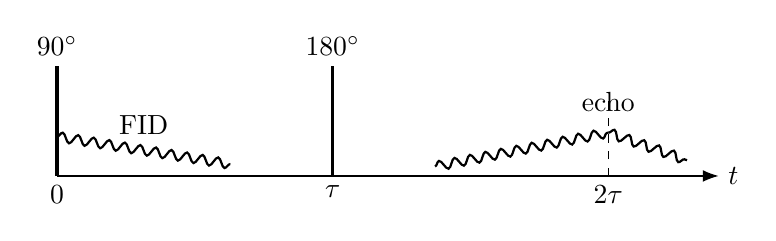
\begin{tikzpicture}[scale=1.0]
\draw[-{Latex[length=2mm]}] (0,0) -- (8.4,0) node[right]{$t$};
\draw[very thick] (0,0) -- (0,1.4); \node[above] at (0,1.4){$90^{\circ}$};
\draw[very thick] (3.5,0) -- (3.5,1.4);
   \node[above] at (3.5,1.4){$180^{\circ}$};
\node[below] at (0,0){$0$};
\node[below] at (3.5,0){$\tau$};
\node[below] at (7.0,0){$2\tau$};
\draw[dashed] (7.0,0) -- (7.0,1.0);
\draw[thick,decorate,decoration={snake,amplitude=0.6mm,segment length=2mm}]
   (0,0.5) -- (2.2,0.15);
\draw[thick,decorate,decoration={snake,amplitude=0.6mm,segment length=2mm}]
   (4.8,0.12) -- (7.0,0.55);
\draw[thick,decorate,decoration={snake,amplitude=0.6mm,segment length=2mm}]
   (7.0,0.55) -- (8.0,0.2);
\node[above] at (7.0,0.7){echo};
\node at (1.1,0.65){FID};
\end{tikzpicture}
\caption{The Hahn spin-echo sequence. A $90^{\circ}$ pulse at $t=0$
initiates the FID; a $180^{\circ}$ refocusing pulse at $t=\tau$ inverts
the accumulated phases; the signal rephases into an echo at $t=2\tau$.
The echo is reduced relative to the initial FID by the irreversible
factor $e^{-2\tau/\Ttwo}$.}
\label{fig:pulse}
\end{figure}

The mechanism is exact for the static part. After the $180^{\circ}$
pulse, nucleus $i$ carries phase
$-\Delta\omega_{i}\tau$ and continues to accumulate at the same rate, so
at $2\tau$ its static phase is
\begin{equation}
-\Delta\omega_{i}\tau+\Delta\omega_{i}(2\tau-\tau)
=-\Delta\omega_{i}\tau+\Delta\omega_{i}\tau=0.
\label{eq:refocus}
\end{equation}
The cancellation is \emph{independent of} $\Delta\omega_{i}$: every
nucleus, whatever its fixed offset, returns to zero phase at $2\tau$
simultaneously. The fan closes; the moments realign; the macroscopic
transverse magnetisation---the observable---reappears.

\subsection{The echo deficit}
\label{sec:deficit}

The echo is not as tall as the original FID. The fluctuating part
\eqref{eq:phifluc} is not cancelled by the pulse, because the random
phase a nucleus accumulates between $\tau$ and $2\tau$ is statistically
independent of what it accumulated between $0$ and $\tau$; inverting the
past phase cannot pre-compensate independent future kicks. The residual
random phase degrades the realignment, and the echo amplitude is reduced
by
\begin{equation}
\frac{A(2\tau)}{A(0)}=e^{-2\tau/\Ttwo},
\label{eq:echodeficit}
\end{equation}
governed by the \emph{true} relaxation time $\Ttwo$, not by $\Tstar$.
Measuring echo height versus $\tau$ isolates $\Ttwo$: the echo subtracts
away the reversible inhomogeneous dephasing and lays bare the
irreversible homogeneous part.

% =====================================================================
\section{The Echo Recovers Configuration, Not History}
\label{sec:configuration}
% =====================================================================

We now formalise the spin echo in the language of
Section~\ref{sec:three-quantities}. The microstate of the spin ensemble
in the rotating frame is the full list of phases
$\Mic(t)=(\varphi_{1}(t),\dots,\varphi_{N}(t))$; the observable is the
normalised transverse magnetisation
\begin{equation}
\Obs(t)=\frac{1}{N}\Bigl|\sum_{i=1}^{N}e^{\,i\varphi_{i}(t)}\Bigr|;
\label{eq:obs}
\end{equation}
and the count is $\Count(t)=ft$ for the spectrometer's reference
oscillator (Theorem~\ref{thm:time-count}).

\begin{theorem}[Echo-Configuration Recovery]
\label{thm:config}
In the Hahn-echo sequence, restricted to the inhomogeneous ($\Tstar$)
dephasing:
\begin{enumerate}[leftmargin=1.7em,label=(\roman*),itemsep=0.2em]
\item the observable returns, $\Obs(2\tau)=\Obs(0)$, by the
$\Delta\omega_{i}$-independent refocusing \eqref{eq:refocus};
\item the microstate is never lost: at every instant
$t\in[0,2\tau]$ each $\varphi_{i}(t)$ is an exactly determined function
of the fixed offset $\Delta\omega_{i}$ and the pulse history, so
$\Mic(t)$ carries the complete information of $\Mic(0)$ forward without
erasure;
\item the count increases monotonically,
$\Count(2\tau)>\Count(\tau)>\Count(0)$, by
Theorem~\ref{thm:monotone}.
\end{enumerate}
Consequently the echo is the construction of a \emph{new} microstate
$\Mic(2\tau)$, reached by strictly forward operations, whose
\emph{observable} happens to coincide with a past observable. No past
microstate is re-occupied and no past count is restored.
\end{theorem}

\begin{proof}
(i) is Equation~\eqref{eq:refocus} summed over the ensemble in
\eqref{eq:obs}. (ii): under inhomogeneous dephasing the phase is
\eqref{eq:phistat} before the pulse and its sign-flipped continuation
after; both are deterministic functions of the fixed $\Delta\omega_{i}$,
a permanent property of nucleus $i$ carried in the microstate, so no
$\varphi_{i}$ is ever undetermined or erased. (iii) is
Theorem~\ref{thm:monotone} over $[0,2\tau]$. The final clause follows:
$\Obs(2\tau)=\Obs(0)$ by (i) while $\Count(2\tau)>\Count(0)$ by (iii),
so by Theorem~\ref{thm:distinct} the coincidence of observables is
neither a recurrence of microstate nor of count.
\end{proof}

\begin{remark}[The decay of the FID is not a loss]
\label{rem:not-loss}
Theorem~\ref{thm:config}(ii) makes precise a point easily missed: the
inhomogeneous decay of the FID is a shrinking of the \emph{observable}
$\Obs$, not a loss of information from the \emph{microstate} $\Mic$. The
moments fan out, the vector sum cancels, the signal vanishes---yet every
phase remains exactly where the deterministic dynamics put it. This is
the many-to-one gap of Definition~\ref{def:three}(ii): a small
observable is compatible with a fully determinate, information-rich
microstate. The echo exploits this gap. It does not retrieve lost
information; it re-aligns information that was never lost.
\end{remark}

Theorem~\ref{thm:config} is the sharpest illustration of why ``the
signal came back'' does not mean ``the system went back.'' In the spin
echo one can point to all three quantities at once: the observable that
returned, the microstate that went forward intact, and the count that
advanced and cannot return. The naive reading collapses them; the
experiment pulls them apart.

% =====================================================================
\section{The Refocusability--Partition Exclusion Theorem}
\label{sec:exclusion}
% =====================================================================

Theorem~\ref{thm:config} was restricted to the inhomogeneous part. We
now explain \emph{why} the refocusing pulse recovers the static
dephasing but is powerless against the fluctuating dephasing. The answer
is a structural exclusion, and it identifies the irreversible part of
relaxation with the count-incrementing part.

\begin{definition}[Partition event]
\label{def:partition-event}
A \emph{partition event} for a constituent is an interaction with other
degrees of freedom (other spins, the lattice, the diffusive environment)
that transfers which-constituent information into those degrees of
freedom and commits it there: after the event, recovering the
constituent's pre-event phase would require reading the correlated state
of the environment, not the constituent alone. Each fluctuating kick
$\delta\omega_{i}(t')\,\mathrm{d}t'$ in \eqref{eq:phifluc} is the phase
imprint of such an event.
\end{definition}

\begin{definition}[Refocusable contribution]
\label{def:refocusable}
A dephasing contribution is \emph{refocusable at $\tau$} if there exists
an operation $P$ applied at $\tau$ (acting on the present microstate
$\Mic(\tau)$) such that the subsequent forward evolution restores the
observable, $\Obs(2\tau)=\Obs(0)$, with respect to that contribution.
\end{definition}

\begin{theorem}[Refocusability--Partition Exclusion]
\label{thm:exclusion}
A dephasing contribution is refocusable at $\tau$ \emph{if and only if}
it created no partition event in $[0,\tau]$. Equivalently: a contribution
is refocusable iff the phase it produces at $2\tau$ is a determinate
function of the present microstate $\Mic(\tau)$; a contribution that
incremented the partition count through committed interactions is, by
construction, not such a function, and is therefore not refocusable.
\end{theorem}

\begin{proof}
($\Leftarrow$) Suppose the contribution created no partition event. Then
no which-spin information was committed to the environment, and the
contribution is a deterministic function of properties carried in the
microstate---for the static offsets, the fixed $\Delta\omega_{i}$. The
future phase increment over $[\tau,2\tau]$ equals the past increment over
$[0,\tau]$, because the generating offset is unchanged. The operation
$P=$ ``$\varphi_{i}\mapsto-\varphi_{i}$'' (the $180^{\circ}$ pulse) then
yields the cancellation \eqref{eq:refocus}, restoring $\Obs$.

($\Rightarrow$) Contrapositive: suppose the contribution created
partition events. By Definition~\ref{def:partition-event} the phase
increment over $[\tau,2\tau]$ is generated by interactions whose realised
values are committed to the environment and are statistically independent
of the increment over $[0,\tau]$; knowing $\Mic(\tau)$ does not determine
the future increment. Any operation $P$ at $\tau$ acts only on
$\Mic(\tau)$; it can negate the accumulated past phase but cannot
pre-compensate an increment that is not a function of $\Mic(\tau)$.
Hence the residual phases at $2\tau$ have non-zero variance, the vector
sum \eqref{eq:obs} is degraded, and $\Obs(2\tau)<\Obs(0)$.
\end{proof}

\begin{corollary}[The echo deficit is the count made visible]
\label{cor:deficit}
The echo-amplitude deficit \eqref{eq:echodeficit},
$1-e^{-2\tau/\Ttwo}$, is a calibrated, directly observed measurement of
the accumulated partition events in $[0,2\tau]$. The reversible part of
relaxation is exactly the configurational ($\Mic$-determined) part; the
irreversible part is exactly the count-incrementing part. The
homogeneous relaxation envelope is the count $\Count$ rendered as a
laboratory signal.
\end{corollary}

This is the structural lock the whole construction needed: the boundary
between what an idealised reversal can and cannot recover coincides
\emph{exactly} with the boundary between the configurational quantities
($\Obs,\Mic$) and the count $\Count$. The experiment does not merely
illustrate the Three-Quantity Separation; it measures the separating
quantity.

% =====================================================================
\section{The Loschmidt Echo Progression and the Irreducible Floor}
\label{sec:progression}
% =====================================================================

The Hahn echo reverses only the inhomogeneous, single-particle dephasing.
A natural research program, pursued for seven decades, asks: how much
more of the dynamics can be reversed if we engineer the refocusing more
ambitiously? The answer is the decisive empirical structure of this
paper.

\begin{description}[leftmargin=0em,itemsep=0.35em]
\item[Hahn echo \citep{hahn1950}.] A single $180^{\circ}$ pulse reverses
static single-spin dephasing. Residual: $e^{-2\tau/\Ttwo}$, set by the
fluctuating environment.

\item[Carr--Purcell--Meiboom--Gill (CPMG)
\citep{carr1954,meiboom1958}.] A \emph{train} of refocusing pulses,
spaced more finely than the correlation time of the fluctuations,
suppresses part of the diffusive and slowly-fluctuating dephasing as
well. The faster the pulsing, the more is recovered---but the recovery
saturates: a residual decay survives, governed by the genuinely fast,
irreducible fluctuations.

\item[Magic echo and many-body reversal
\citep{rhim1971}.] By engineering the radio-frequency drive one can
effectively invert the sign of the \emph{dipolar coupling Hamiltonian}
itself, $H\to-H$, reversing not just single-spin precession but the
many-body interacting evolution. This is the closest physical
approximation to Loschmidt's ``reverse all velocities'' ever realised.

\item[Polarization / Loschmidt echo
\citep{levstein1998,jalabert2001,gorin2006}.] The most refined
many-body reversal experiments measure the \emph{fidelity} with which the
reversed evolution reconstructs the initial state. As the engineered
reversal is made ever more perfect, the reconstruction fidelity does not
approach unity. It approaches a floor whose decay rate becomes
\emph{independent of the perturbation strength}---set by the system's own
internal dynamics rather than by the residual imperfection of the
engineering \citep{jalabert2001,gorin2006}.
\end{description}

\begin{principle}[The irreducible floor]
\label{prin:floor}
Across the progression, improved engineering of the reversal exposes an
engineering-independent floor. The better one approximates Loschmidt's
operation, the more sharply one isolates a residual irreversibility that
does not diminish with further engineering, because it is not an artifact
of imperfect control but the signature of accumulated partition events.
\end{principle}

\begin{theorem}[Floor unification]
\label{thm:floor}
The irreducible floor of the Loschmidt-echo progression is a single
object viewed three ways: (a) the homogeneous-relaxation limit
$e^{-2\tau/\Ttwo}$ of the configurational recovery
(Corollary~\ref{cor:deficit}); (b) the non-decrementability of the
partition count (Theorem~\ref{thm:incoherence}); (c) the positivity of
the smallest committed correlation that any refocusing operation, acting
only on the present microstate, cannot pre-compensate
(Theorem~\ref{thm:exclusion}).
\end{theorem}

\begin{proof}
(a)$\Leftrightarrow$(c): by Theorem~\ref{thm:exclusion} the
non-refocusable part is precisely the partition-event part, whose
envelope is \eqref{eq:echodeficit}; the floor is that envelope's
non-vanishing as engineering improves, because partition events, once
committed, are not functions of the present microstate.
(c)$\Leftrightarrow$(b): a partition event is, by
Definition~\ref{def:partition-event}, a committed increment of $\Count$;
by Theorem~\ref{thm:incoherence} no operation decrements $\Count$, so no
refocusing can annul a committed event. The three descriptions therefore
have the same content: a positive floor exists iff at least one partition
event has been committed, and the count records exactly those.
\end{proof}

The lab has been running Loschmidt's own experiment for seventy years.
Every refinement confirms the floor. \emph{The experiment named after
Loschmidt refutes Loschmidt's premise:} the more completely one engineers
the reversal, the more cleanly one measures the quantity that cannot be
reversed.

% =====================================================================
\section{No Reverse Operation Exists}
\label{sec:operations}
% =====================================================================

The arguments so far live within the framework of dynamical
systems---state spaces, flows, trajectories as curves. We now move to a
deeper level. Real physical processes are not curves in continuous phase
space; they are sequences of physical \emph{operations}, each
constitutively one-way.

\begin{definition}[Operation; constitutively one-way]
\label{def:operation}
A physical \emph{operation} $\Op:\Gamma\to\Gamma$ is a partial map
between observable states implemented by a specific physical mechanism;
different mechanisms producing the same input--output map are different
operations. An operation $\Op$ is \emph{constitutively one-way} if no
operation $\Op^{*}$ exists in physical reality such that
$\Op^{*}\circ\Op=\mathrm{id}$ \emph{as physical processes} (not merely as
mathematical maps).
\end{definition}

The empirical world is full of constitutively one-way operations.
Fertilisation has no mechanism called ``un-fertilisation''; combustion
has no single reverse operation (reduction, photosynthesis, and
electrolysis are different operations with different intermediates);
mitosis is not run backwards by cell fusion (a different mechanism);
crystallisation is not dissolution-in-reverse. Consider a maize seed in
your hand. ``How was this produced?'' is a coherent question with a
determinate answer: pollination, fertilisation, zygote and endosperm
formation, mitotic division, differentiation, starch accumulation,
dehydration, dormancy. ``Can this be reached by reversing time?'' is
incoherent: each constituent operation has no reverse mechanism, only
different forward operations whose mathematical action happens to match
an inverse. The seed is the end-product of a sequence of constitutively
one-way operations; its existence in your hand is testimony to their
directionality.

\begin{theorem}[Constitutive Asymmetry]
\label{thm:constitutive}
Every physical trajectory is a sequence of operations
$\{\Op_{1},\dots,\Op_{k}\}$, each constitutively one-way. The composite
has no reverse trajectory in the operational sense: no sequence of
operations exists whose enactment undoes the forward trajectory as a
physical process.
\end{theorem}

\begin{proof}[Sketch]
Suppose a reverse trajectory
$\widetilde{\Op}_{1}\circ\cdots\circ\widetilde{\Op}_{k}$ existed,
composing to the identity-as-a-process. Then each $\widetilde{\Op}_{i}$
inverts $\Op_{i}$ as a process. Three cases. If $\widetilde{\Op}_{i}$
does not exist, the reverse is unavailable. If it exists but is a
different operation, it has different mechanism and intermediates, so
$\widetilde{\Op}_{i}\circ\Op_{i}$ is a sequence of two distinct
operations, not the identity-as-a-process. If it exists and is the same
operation, $\Op_{i}$ is its own inverse---possible only for symmetry
transformations that do not advance the partition structure, which
generic operations (ionisation, detection, fertilisation) are not. In
all generic cases the reverse trajectory does not exist as a physical
process.
\end{proof}

\begin{corollary}[Reversibility is a coarse-graining artifact]
\label{cor:coarse}
The time-reversibility of the continuous-flow description
$\dot{x}=f(x,t)$ is an artifact of replacing operation-sequences with
continuous flows. The flow averages over the operational structure, and
the averaging happens to be invariant under $t\to-t$. The averaging is
not itself a physical process.
\end{corollary}

\begin{principle}[Rewind-as-Forward]
\label{prin:rewind}
A ``rewound'' sequence is not the original sequence run backward. It is a
new forward sequence whose state-content is the reverse-ordered list of
states from the original. The rewinding itself is a forward operation
that increments the global partition count.
\end{principle}

A film projector showing a movie in reverse runs forward in time as it
does so: photons are emitted forward, the audience perceives them
forward, the operator's watch ticks forward. The frames appear in reverse
order, but the reverse-ordering is a forward physical process. The same
holds for every claimed time-reversal in physics. A Maxwell demon
reversing molecular velocities must act forward, measure forward, expend
forward thermodynamic resources; the ``reversed'' trajectory that ensues
is a new forward trajectory whose state-content mimics the reverse
ordering of the original states. By Theorem~\ref{thm:constitutive} the
operations constituting it are not the inverses of the original
operations; by Principle~\ref{prin:rewind} their enactment increments the
count.

\begin{remark}[Solution sets versus physical processes]
\label{rem:levels}
The mathematical operation $T:x(t)\mapsto x(-t)$ is well defined as an
automorphism of the solution set: it sends a solution to a solution, no
more problematic than sending $f(x)$ to $f(-x)$ on a function space. But
it does not correspond to a physical operation on a system; there is no
laboratory procedure whose enactment maps a system from $x(t)$ to
$x(-t)$. The mathematical operation acts on representations; physical
operations act on systems. The conflation of these two levels is the
source of Loschmidt's paradox (Corollary~\ref{cor:category}).
\end{remark}

% =====================================================================
\section{Causal Distinguishability: An Independent Corollary}
\label{sec:causal}
% =====================================================================

The preceding depths resolve the paradox without any appeal to observers.
We record here a fourth, independent route to the same conclusion, useful
because it needs nothing of the partition machinery---only the causal
structure of spacetime.

\begin{definition}[Causal partition]
\label{def:causal}
For an event $E$, the \emph{causal partition} divides states into those
causally downstream of $E$ (with $E$ in their past light cone) and those
not. A state at spacetime point $x$ is downstream of $E$ at $y$ iff $y$
lies in the past light cone of $x$.
\end{definition}

\begin{theorem}[Causal distinguishability]
\label{thm:causal}
Let $E_{\mathrm{rev}}$ be the velocity-reversal event at time $T$, let
$S_{0}$ be the state at the initial time $t_{0}<T$, and let $S_{0}'$ be
the post-reversal state at $2T$ whose configuration matches $S_{0}$. Then
$E_{\mathrm{rev}}$ is in the past light cone of $S_{0}'$ but not of
$S_{0}$; the two states lie on opposite sides of the causal partition and
are therefore distinct, independent of any observer.
\end{theorem}

\begin{proof}
$S_{0}$ occurs before $E_{\mathrm{rev}}$ ($t_{0}<T$), so $E_{\mathrm{rev}}$
is not in its past light cone: $S_{0}$ is not downstream of the reversal.
$S_{0}'$ occurs after $E_{\mathrm{rev}}$ ($2T>T$) and the system reached
it by evolving through $E_{\mathrm{rev}}$, so $E_{\mathrm{rev}}$ is in its
past light cone: $S_{0}'$ is downstream. Lying on opposite sides of the
causal partition, $S_{0}\neq S_{0}'$.
\end{proof}

The matching configuration at $2T$ is not a return to $t_{0}$; it is a
distinct state at a later time, carrying the reversal event in its causal
past. This is the same conclusion as Theorem~\ref{thm:config}---the
observable coincides while the history does not---reached now from
spacetime geometry alone.

\begin{remark}[Velocity through zero, and the double occupation]
\label{rem:vzero}
A continuous velocity reversal passes the velocity through $v=0$ at the
turning point, and the procedure is claimed to return the system to its
initial configuration. A genuine return would make the initial state
occur \emph{twice}---once at the start, once on return at a strictly
later count. By Theorem~\ref{thm:monotone} the later occurrence carries a
strictly greater count, so the two occurrences are distinct states with
the same configuration, never the same state revisited. The nearest
genuine recurrence of a configuration lies a full oscillatory period
later (Proposition~\ref{prop:osc}); it is a forward advance to a
resembling configuration, not a return to the original moment.
\end{remark}

% =====================================================================
\section{Objections and Replies}
\label{sec:objections}
% =====================================================================

\paragraph{``But the equations \emph{are} time-reversible.''}
Granted, and irrelevant. Time-reversal invariance \eqref{eq:trinv} is a
property of the solution set (Remark~\ref{rem:hinge}). The claim of this
paper is not that the equations lack the symmetry but that the symmetry
is not an operation---there is no physical procedure whose enactment
realises $R$ on a system (Corollary~\ref{cor:category},
Remark~\ref{rem:levels}). The mathematics is untouched; only its
operational interpretation is corrected.

\paragraph{``The spin echo really does reverse the dynamics.''}
It does not. By Theorem~\ref{thm:config} the echo recovers the
\emph{observable} by a forward operation on a \emph{preserved} microstate
while the \emph{count} advances; nothing is run backward. The very part
of the evolution that \emph{is} a committed dynamical process---the
homogeneous, partition-event part---is precisely the part the echo
cannot recover (Theorem~\ref{thm:exclusion}). The echo is the cleanest
possible demonstration that ``the signal returned'' is not ``the system
went back.''

\paragraph{``In a block universe all moments coexist; there is no
flow to reverse.''}
The account here is neutral on the metaphysics of becoming. Whether or
not all moments ``coexist,'' the operational quantity $\Count$ is
monotone along every worldline (Theorem~\ref{thm:monotone}) and no
operation decrements it (Theorem~\ref{thm:incoherence}). The eternalist
may read $\Count$ as a monotone labelling of events along a worldline
rather than a flowing now; the conclusion---no operation realises
decrement---is unchanged.

\paragraph{``The continuum limit $f\to\infty$ erases the discreteness
you rely on.''}
The continuum parameter $t$ is the $f\to\infty$ idealisation of the count
(Theorem~\ref{thm:time-count}); taking the limit does not make the count
decrementable, it only makes its steps unresolvably fine. Monotonicity
survives every finite $f$ and its limit. The discreteness is a
convenience of exposition, not a premise of the argument.

\paragraph{``This is just Boltzmann's improbability restated.''}
No. Boltzmann grants that reversal is possible and explains why it is not
seen (Table~\ref{tab:standard}). The present claim is stronger and
different in kind: reversal is not improbable but \emph{incoherent as an
operation} (Theorem~\ref{thm:incoherence}), and this is witnessed, not
merely argued, by the irreducible floor of the echo progression
(Theorem~\ref{thm:floor}).

% =====================================================================
\section{Falsifiable Predictions}
\label{sec:predictions}
% =====================================================================

The account is empirical, not merely interpretive, and makes definite
predictions.

\begin{enumerate}[leftmargin=1.5em,itemsep=0.3em]
\item \textbf{Engineering-independence of the floor.} In any
many-body reversal experiment, as control imperfections are reduced, the
residual fidelity-decay rate approaches a positive limit set by the
system's intrinsic dynamics and \emph{independent} of the residual
perturbation strength (Principle~\ref{prin:floor}). A reversal protocol
whose residual decay vanished with improving control would falsify the
account.

\item \textbf{Floor--$\Ttwo$ identity.} The Hahn-echo floor is
$e^{-2\tau/\Ttwo}$ with $\Ttwo$ the homogeneous relaxation time measured
independently; the count-deficit $1-e^{-2\tau/\Ttwo}$ must track the
independently measured population of committed partition events
(Corollary~\ref{cor:deficit}). A discrepancy between the echo deficit and
the independently measured homogeneous relaxation would falsify the
identification.

\item \textbf{Positivity of the smallest knowable error.} No bounded
observer's reconstruction of an initial state by engineered reversal can
have strictly zero error; the minimum is set by the smallest committed
correlation not pre-compensable from the present microstate
(Theorem~\ref{thm:exclusion}). A demonstrated zero-error reversal of a
genuinely interacting many-body evolution would falsify the account.
\end{enumerate}

% =====================================================================
\section{Discussion}
\label{sec:discussion}
% =====================================================================

\paragraph{Reversible computing.} Even logically reversible gates
\citep{bennett1973}, and the Landauer bound on erasure
\citep{landauer1961}, operate within the count: executing a reversible
gate is a forward operation incrementing $\Count$
(Theorem~\ref{thm:inverse}). Reversible computing minimises the
$\Mic$-level entropy generated per logical step; it cannot make the
global count decrement, and so cannot run time backward.

\paragraph{Measurement.} A measurement commits which-system information
to an apparatus---a partition event in the sense of
Definition~\ref{def:partition-event}. The irreversibility of measurement
is then not an extra postulate but an instance of
Theorem~\ref{thm:exclusion}: the committed correlation is not a function
of the system's present microstate alone and cannot be refocused away.

\paragraph{Quantum chaos.} The Loschmidt-echo / fidelity-decay literature
\citep{jalabert2001,gorin2006} already measures, under another name,
exactly the separating quantity of Theorem~\ref{thm:floor}. The
perturbation-independent decay regime is the floor; our account predicts
its positivity and identifies it with the committed partition count.

\paragraph{The arrow of time.} On this account the arrow is neither
imposed by special initial conditions \citep{penrose1989} nor a matter of
coarse-graining \citep{gibbs1902} nor of ignorance \citep{jaynes1957}. It
is constitutive: time \emph{is} the monotone count
(Theorem~\ref{thm:time-count}), and the count cannot decrease because
counting is what time is (Theorem~\ref{thm:incoherence}).

% =====================================================================
\section{Conclusion}
\label{sec:conclusion}
% =====================================================================

Loschmidt's paradox asks how the time-reversal invariance of the
microscopic equations can coexist with the irreversibility of the
macroscopic world. We have argued that the question is malformed, and we
have argued it at four depths, each independently sufficient and each
sharper than the last.

\emph{Time is a count} (Section~\ref{sec:partition}): elapsed time is the
monotone partition count $\Count$, no operation decrements it, and the
mathematical time-reversal map acts on representations rather than
systems---so ``is physical dynamics reversible?'' is a category error.
\emph{The paradox feeds on a conflation}
(Section~\ref{sec:three-quantities}): it identifies the observable, the
microstate, and the count, which are logically independent; once they are
separated, a Poincar\'e recurrence is seen to return the microstate but
never the count, dissolving the Zermelo objection. \emph{The separation
is witnessed in the laboratory}
(Sections~\ref{sec:nmr}--\ref{sec:progression}): the spin echo recovers
the observable by a forward operation on a preserved microstate while the
count advances, and the seventy-year progression of reversal experiments
exposes an irreducible, engineering-independent floor that is the count
made visible. \emph{No reverse operation exists}
(Section~\ref{sec:operations}): physical trajectories are sequences of
constitutively one-way operations, the reversibility of the flow
description is a coarse-graining artifact, and every ``rewind'' is a
forward operation incrementing the count.

The Second Law is, on this account, not a statistical regularity
overlaid on reversible foundations but the operational signature of what
time is. The completion of the resolution is therefore not a stronger
argument but an empirical fact: the experiment named after Loschmidt has
been refuting Loschmidt's premise since 1950.

% =====================================================================
\bibliographystyle{plainnat}
\bibliography{references}
% =====================================================================

\end{document}
